
\tikzset{every picture/.style={line width=0.75pt}} %set default line width to 0.75pt        

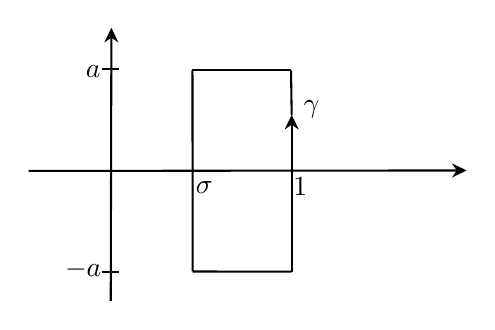
\begin{tikzpicture}[x=0.75pt,y=0.75pt,yscale=-1,xscale=1]
%uncomment if require: \path (0,300); %set diagram left start at 0, and has height of 300

%Straight Lines [id:da9604484458166531] 
\draw [line width=0.75]    (98.52,143) -- (98.83,14.33) ;
\draw [shift={(98.84,11.33)}, rotate = 90.14] [fill={rgb, 255:red, 0; green, 0; blue, 0 }  ][line width=0.08]  [draw opacity=0] (7.14,-3.43) -- (0,0) -- (7.14,3.43) -- (4.74,0) -- cycle    ;
%Straight Lines [id:da7824602823917455] 
\draw [line width=0.75]    (59,80.3) -- (267,80.07) ;
\draw [shift={(270,80.07)}, rotate = 179.94] [fill={rgb, 255:red, 0; green, 0; blue, 0 }  ][line width=0.08]  [draw opacity=0] (7.14,-3.43) -- (0,0) -- (7.14,3.43) -- (4.74,0) -- cycle    ;
%Straight Lines [id:da1843809737858978] 
\draw    (94.38,31.3) -- (102.67,31.3) ;
%Straight Lines [id:da005604616839814391] 
\draw    (94.38,129.07) -- (102.67,129.07) ;
%Straight Lines [id:da7882221024941302] 
\draw    (137.89,31.88) -- (185.38,31.88) ;
%Straight Lines [id:da6837927780552461] 
\draw    (137.89,31.88) -- (138,128.75) ;
%Straight Lines [id:da1843879383978263] 
\draw    (138,128.75) -- (185.7,128.83) ;
%Straight Lines [id:da7511938377361984] 
\draw    (185.7,128.83) -- (185.7,56.25) ;
\draw [shift={(185.7,53.25)}, rotate = 90] [fill={rgb, 255:red, 0; green, 0; blue, 0 }  ][line width=0.08]  [draw opacity=0] (7.14,-3.43) -- (0,0) -- (7.14,3.43) -- (4.74,0) -- cycle    ;
%Straight Lines [id:da0698707153553133] 
\draw    (185.7,53.25) -- (185.38,31.88) ;

% Text Node
\draw (190,45) node [anchor=north west][inner sep=0.75pt]    {$\gamma $};
% Text Node
\draw (138,84) node [anchor=north west][inner sep=0.75pt]    {$\sigma $};
% Text Node
\draw (185,82) node [anchor=north west][inner sep=0.75pt]    {$1$};
% Text Node
\draw (85,28) node [anchor=north west][inner sep=0.75pt]    {$a$};
% Text Node
\draw (75,122) node [anchor=north west][inner sep=0.75pt]    {$-a$};

\end{tikzpicture}